\section{RATIONALE ON THE COMBINATION BETWEEN VISUALIZATION AND DATA CLUSTERING}\label{sec:rationale}%

In many cases, the analyst, with some knowledge of a system, can perform an analysis of the results and create a concise final model. However, especially for complex systems, it is necessary to use strategies to correctly interpret the results. Such strategies involve the observation of repeated patterns and identification of architectural violations in the source code.

In general, automatic architecture reconstruction methods, such as clustering techniques, have the advantage to produce different models for a single software system in a short period of time. Such models can be constructed differently by changing configuration settings on clustering algorithm used during the process. Through the analysis of different models it is possible to identify patterns that recur frequently in the results. One of the most prominent software clustering tool is Bunch~\cite{mitchell_heuristic_2002}, which transforms the architecture recovery problem into an optimization problem. Bunch uses hill-climbing and genetic algorithms to find the software cluster partitions that maximizes the modularization quality.  %Bunch provides the Nearest Ascent Hill Climbing (NAHC) as default.

However, when the idea is not clear of how the system structure is composed, the various models produced by clustering process may not suffice to understand the complex software \cite{craft}, since the results show a high level view of the architecture. In this sense, the use of software visualization techniques allow a fine-grained observation of different outcomes on a low level of abstraction. By means of interactive operations in the models produced by the visualization software, it is possible to decompose components of the system in more detailed representations. Thus, allowing the observation of concepts as part of the architecture in greater depth. In this context, linking the models produced by the clustering process with the model produced by the software visualization process, it is possible to get different representations of the system to form a final model with greater precision. 

We illustrate how this approach can be performed by taking into account the results shown in Figure \ref{exemplo_comparacao_modelos}. Assuming that the process of obtaining architecture models recovered four different results, through the use of software visualization techniques and software clustering algorithms. Each model features nine entities, namely: \{1,2,3,4,5,6,7,8,9\}. \replaced{The ratio of the frequency the entities were classified as part of the same group is observed in Table \ref{ocorrencias_1}.}{By performing a count of the grouped entities it is  possible to obtain the ratio of how many times the entity was classified similarly to the other. The result of this count is observed in Table \ref{ocorrencias_1}.}

\begin{table}[h]
	\centering
	\caption{Occurrences of entities in the results.}
	\label{ocorrencias_1}
	\begin{tabular}{|cc|}
		\hline
		\multicolumn{1}{|l}{Relation} & \multicolumn{1}{l|}{Occurrence} \\ \hline
		\{1,2,3\},\{7,8,9\}                  & 100\%                           \\ \hline
		\{4,5\}, \{6,7,8,9\}                    & 50\%                          \\ \hline
		\{1,2,3,4\},\{4,5,6\},\{5\},\{6\}                  & 25\%           \\ \hline
	\end{tabular}
\end{table}

By analyzing the results in Table~\ref{ocorrencias_1}, it is possible to see that entities \{1,2,3\} can be classified into a single module, since they appear 100\% of the times in the same cluster; so do the entities \{7,8,9\}. In many cases, the aggregation of results provide technical assistance, by highlighting the common patterns. It is possible to gain confidence that agreement across a collection of results can reflect the system structure \cite{craft}. On the other hand, entities \{4,5,6\} may be classified either as a single module or scattered into different modules, since there is no agreement between the results. In such situations, additional analysis must be performed for each entity. \deleted{This simple example illustrates how to use different results to help the composition of a single final model.}

\begin{figure}[!h]
	\centering
	\includegraphics[width=0.35\textwidth]{exemplo_comparacao_modelos_en_novo}
	\caption{Different results for comparison.}
	\label{exemplo_comparacao_modelos}
\end{figure}

However, a more careful analysis of the results may reveal that other factors may influence the final model produced by clustering and visualization software techniques. A software system throughout its life cycle is susceptible to several changes in its architecture. However, such operations can introduce architectural violations in the code, for example, violation of the layers, break of abstractions or feature duplication \cite{kazman_view_1998}. In this context, reverse engineering methods are strongly affected by those shortcomings in the system code base~\cite{Platenius_2012}.  Such violations should be identified and addressed, so the correctness of the final model should not be affected.

To illustrate an architecture violation, we will use the results of Figure \ref{3_exemploMatrizViolada}, which depicts a representation of architecture components through a dependency structure matrix (DSM). The figure depicts how the interaction works. The software elements are numbered from 1 to 9, where, for example, the module 1 requires information from module 2. On the other hand, the figure shows also that the module 4 provides information to the module 5. This relationship is violated by module 5, since it uses resources of the module 4, characterizing an architectural violation. Removing such violation, the modularization results would likely change. 

 \begin{figure}[!h]
 	\centering
 	\includegraphics[width=0.3\textwidth]{3_exemploMatrizViolada_en_novo}
 	\caption{DSM representation	of dependences.}
 	\label{3_exemploMatrizViolada}
 \end{figure}
 
\deleted{ Assuming entity 4 is wrongly mapped as part of a module. This happens due to a coupling between entities 4 and 5, which illustrates an architecture violation. All results would be classified differently if such violation was removed, as shown in Figure \ref{exemplo_comparacao_modelos2}.} Table \ref{ocorrencias_2} presents the results of the new analysis, taking into account the aggregation of similar entities after the identified architecture violation was removed. Analyzing the results, it is possible to check the impact of the violation. The module containing the first mapping \{1,2,3\} now adds entity 4 in 100\% of the times as part of the same module. As for the mapping \{5,6\} there is also a higher chance of being classified in a same module, as both entities occur as part of the same module with higher frequency after the architecture violation was detected and removed.


\begin{table}[]
	\centering
	\caption{Occurrences of entities between the results after elimination of architectural violation}
	\label{ocorrencias_2}
	\begin{tabular}{|ll|}
		\hline
		\multicolumn{1}{|l}{Relation} & \multicolumn{1}{l|}{Occurrence} \\ \hline
		\{1,2,3,4\}, \{7,8,9\}  	 & 100\%                           \\ \hline
		\{5\}, \{5,6\}	& 50\%                            \\ \hline
		\{6\}, \{6,7,8,9\}	& 25\%                            \\ 
		\hline
	\end{tabular}
\end{table}

%\begin{figure}[!h]
%	\centering
%	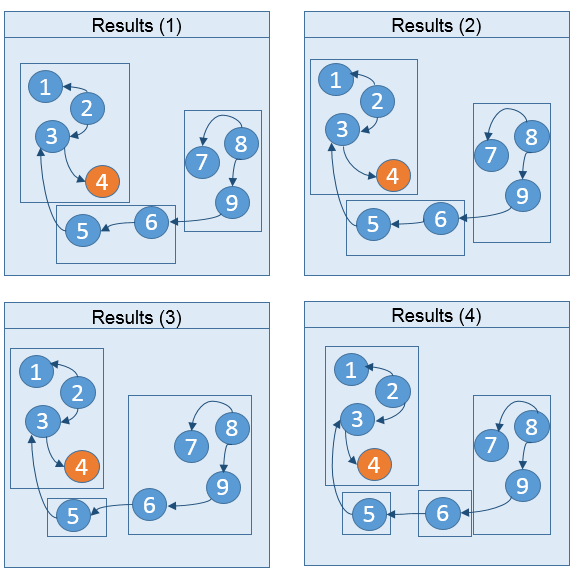
\includegraphics[width=0.43\textwidth]{exemplo_comparacao_modelos_2_en}
%	\caption{Eliminating the architectural violation of results.}
%	\label{exemplo_comparacao_modelos2}
%\end{figure}

\deleted{Such violations can be found through an analysis of the artifacts produced by software visualization. As an example, take into account the dependency structure matrix shown previously in Figure \ref{3_exemploMatrizViolada}. Through observation of the DSM, it is possible to note a relationship exists between layers, and each layer depends on the upper layers. However, this relationship is violated by layer "Date" (4), since it uses resources of the layer  "View" (1), characterizing an architectural violation. Once the violation is detected, it should be treated as failure and, if necessary, modify the data set for the clustering process, so that the relationship is not considered. Thus, avoiding the production of wrong models that may affect the interpretation of the results.}

By these means, we propose to promote how practitioners may obtain more accurate architecture recovery process by interweaving complementary levels of abstraction provided by architecture recovery techniques. If a higher level of abstraction is needed, software clustering via Bunch tool, for exemple, allows the user to choose the number of clusters of the recovered architecture. This information could then be refined and verified by applying semi-automatic techniques, provided by tools like~\cite{VBDepend, Architexa, X-Ray}. On the other hand, we claim that the order of which technique to start with should not influence the accuracy of the architecture recovery due to the complementary level of information each technique provides. In the next section, we evaluate not only such claim, but also the validity of our proposal.